\documentclass[journal,12pt,twocolumn]{IEEEtran}
%
\usepackage{setspace}
\usepackage{gensymb}
\usepackage{xcolor}
%\usepackage{esint}
\usepackage{caption}
%\usepackage{subcaption}
%\doublespacing
\singlespacing
\usepackage{multicol}

\usepackage{iithtlc}
%\usepackage{graphicx}
%\usepackage{amssymb}
%\usepackage{relsize}
\usepackage[cmex10]{amsmath}
\usepackage{mathtools}
%\usepackage{amsthm}
%\interdisplaylinepenalty=2500
%\savesymbol{iint}
%\usepackage{txfonts}
%\restoresymbol{TXF}{iint}
%\usepackage{wasysym}
\usepackage{amsthm}
\usepackage{mathrsfs}
\usepackage{txfonts}
\usepackage{stfloats}
\usepackage{cite}
\usepackage{cases}
\usepackage{subfig}
%\usepackage{xtab}
\usepackage{longtable}
\usepackage{multirow}
%\usepackage{algorithm}
%\usepackage{algpseudocode}
\usepackage{enumitem}
\usepackage{mathtools}
%\usepackage{stmaryrd}

\usepackage{listings}
%    \usepackage[latin]{inputenc}                                 %%
    \usepackage{color}                                            %%
    \usepackage{array}                                            %%
    \usepackage{longtable}                                        %%
    \usepackage{calc}                                             %%
    \usepackage{multirow}                                         %%
    \usepackage{hhline}                                           %%
    \usepackage{ifthen}                                           %%
  %optionally (for landscape tables embedded in another document): %%
    \usepackage{lscape}     
%\usepackage{tikz}
%\usepackage{tkz-euclide}
%\usetkzobj{all}
%%\usepackage[utf8]{inputenc}
%\usepackage{rotating}
%\usetikzlibrary{arrows,shapes,decorations.markings,positioning}
%\usepackage{amsmath}
%\usepackage{ulem}
%\usepackage{soul}

%\usepackage{wasysym}
%\newcounter{MYtempeqncnt}
\DeclareMathOperator*{\Res}{Res}
%\renewcommand{\baselinestretch}{2}
\renewcommand\thesection{\arabic{section}}
\renewcommand\thesubsection{\thesection.\arabic{subsection}}
\renewcommand\thesubsubsection{\thesubsection.\arabic{subsubsection}}

\renewcommand\thesectiondis{\arabic{section}}
\renewcommand\thesubsectiondis{\thesectiondis.\arabic{subsection}}
\renewcommand\thesubsubsectiondis{\thesubsectiondis.\arabic{subsubsection}}

%\DeclareUnicodeCharacter{01B5}{\zst}
%\DeclareRobustCommand\zst{%
%\unskip\nobreak\thinspace\zbar\allowbreak\thinspace\ignorespaces}
%\newcommand{\zbar}{\raisebox{0.2ex}{--}\kern-0.6em Z}


% correct bad hyphenation here
\hyphenation{op-tical net-works semi-conduc-tor}

\def\inputGnumericTable{}  

\lstset{
language=python,
frame=single, 
breaklines=true
}

\begin{document}
%

\theoremstyle{definition}
\newtheorem{theorem}{Theorem}[section]
\newtheorem{problem}{Problem}
\newtheorem{proposition}{Proposition}[section]
\newtheorem{lemma}{Lemma}[section]
\newtheorem{corollary}[theorem]{Corollary}
\newtheorem{example}{Example}[section]
\newtheorem{definition}{Definition}[section]
%\newtheorem{algorithm}{Algorithm}[section]
%\newtheorem{cor}{Corollary}
\newcommand{\BEQA}{\begin{eqnarray}}
\newcommand{\EEQA}{\end{eqnarray}}
\newcommand{\define}{\stackrel{\triangle}{=}}

\bibliographystyle{IEEEtran}
%\bibliographystyle{ieeetr}



\providecommand{\pr}[1]{\ensuremath{\Pr\left(#1\right)}}
\providecommand{\qfunc}[1]{\ensuremath{Q\left(#1\right)}}
\providecommand{\sbrak}[1]{\ensuremath{{}\left[#1\right]}}
\providecommand{\lsbrak}[1]{\ensuremath{{}\left[#1\right.}}
\providecommand{\rsbrak}[1]{\ensuremath{{}\left.#1\right]}}
\providecommand{\brak}[1]{\ensuremath{\left(#1\right)}}
\providecommand{\lbrak}[1]{\ensuremath{\left(#1\right.}}
\providecommand{\rbrak}[1]{\ensuremath{\left.#1\right)}}
\providecommand{\cbrak}[1]{\ensuremath{\left\{#1\right\}}}
\providecommand{\lcbrak}[1]{\ensuremath{\left\{#1\right.}}
\providecommand{\rcbrak}[1]{\ensuremath{\left.#1\right\}}}
\theoremstyle{remark}
\newtheorem{rem}{Remark}
\newcommand{\sgn}{\mathop{\mathrm{sgn}}}
\providecommand{\abs}[1]{\left\vert#1\right\vert}
\providecommand{\res}[1]{\Res\displaylimits_{#1}} 
\providecommand{\norm}[1]{\lVert#1\rVert}
\providecommand{\mtx}[1]{\mathbf{#1}}
\providecommand{\mean}[1]{E\left[ #1 \right]}
\providecommand{\fourier}{\overset{\mathcal{F}}{ \rightleftharpoons}}
%\providecommand{\hilbert}{\overset{\mathcal{H}}{ \rightleftharpoons}}
\providecommand{\system}{\overset{\mathcal{H}}{ \longleftrightarrow}}
\providecommand{\gauss}[2]{\mathcal{N}\ensuremath{\left(#1,#2\right)}}
	%\newcommand{\solution}[2]{\textbf{Solution:}{#1}}
\newcommand{\solution}{\noindent \textbf{Solution: }}
\providecommand{\dec}[2]{\ensuremath{\overset{#1}{\underset{#2}{\gtrless}}}}
%\numberwithin{equation}{section}
%\numberwithin{problem}{section}
\makeatletter
\@addtoreset{figure}{problem}
\makeatother

\let\StandardTheFigure\thefigure
%\renewcommand{\thefigure}{\theproblem.\arabic{figure}}
\renewcommand{\thefigure}{\theproblem}

\def\putbox#1#2#3{\makebox[0in][l]{\makebox[#1][l]{}\raisebox{\baselineskip}[0in][0in]{\raisebox{#2}[0in][0in]{#3}}}}
     \def\rightbox#1{\makebox[0in][r]{#1}}
     \def\centbox#1{\makebox[0in]{#1}}
     \def\topbox#1{\raisebox{-\baselineskip}[0in][0in]{#1}}
     \def\midbox#1{\raisebox{-0.5\baselineskip}[0in][0in]{#1}}


% paper title
% can use linebreaks \\ within to get better formatting as desired
\title{
\logo{
Complex Analysis in Electrical Engineering
}
}
%
%
% author names and IEEE memberships
% note positions of commas and nonbreaking spaces ( ~ ) LaTeX will not break
% a structure at a ~ so this keeps an author's name from being broken across
% two lines.
% use \thanks{} to gain access to the first footnote area
% a separate \thanks must be used for each paragraph as LaTeX2e's \thanks
% was not built to handle multiple paragraphs
%

%\author{Y Aditya, A Rathnakar and G V V Sharma$^{*}$% <-this % stops a space
\author{G V V Sharma$^{*}$% <-this % stops a space
\thanks{*The author is with the Department
of Electrical Engineering, Indian Institute of Technology, Hyderabad
502205 India e-mail:  gadepall@iith.ac.in.All content in this manual is released under GNU GPL.  Free and open source.}% <-this % stops a space
%\thanks{J. Doe and J. Doe are with Anonymous University.}% <-this % stops a space
%\thanks{Manuscript received April 19, 2005; revised January 11, 2007.}}
}
% note the % following the last \IEEEmembership and also \thanks - 
% these prevent an unwanted space from occurring between the last author name
% and the end of the author line. i.e., if you had this:
% 
% \author{....lastname \thanks{...} \thanks{...} }
%                     ^------------^------------^----Do not want these spaces!
%
% a space would be appended to the last name and could cause every name on that
% line to be shifted left slightly. This is one of those "LaTeX things". For
% instance, "\textbf{A} \textbf{B}" will typeset as "A B" not "AB". To get
% "AB" then you have to do: "\textbf{A}\textbf{B}"
% \thanks is no different in this regard, so shield the last } of each \thanks
% that ends a line with a % and do not let a space in before the next \thanks.
% Spaces after \IEEEmembership other than the last one are OK (and needed) as
% you are supposed to have spaces between the names. For what it is worth,
% this is a minor point as most people would not even notice if the said evil
% space somehow managed to creep in.



% The paper headers
%\markboth{Journal of \LaTeX\ Class Files,~Vol.~6, No.~1, January~2007}%
%{Shell \MakeLowercase{\textit{et al.}}: Bare Demo of IEEEtran.cls for Journals}
% The only time the second header will appear is for the odd numbered pages
% after the title page when using the twoside option.
% 
% *** Note that you probably will NOT want to include the author's ***
% *** name in the headers of peer review papers.                   ***
% You can use \ifCLASSOPTIONpeerreview for conditional compilation here if
% you desire.




% If you want to put a publisher's ID mark on the page you can do it like
% this:
%\IEEEpubid{0000--0000/00\$00.00~\copyright~2007 IEEE}
% Remember, if you use this you must call \IEEEpubidadjcol in the second
% column for its text to clear the IEEEpubid mark.



% make the title area
\maketitle

%\tableofcontents

\begin{abstract}
This manual provides applications of Complex Analysis in Electrical Engineering.
%
\end{abstract}
% IEEEtran.cls defaults to using nonbold math in the Abstract.
% This preserves the distinction between vectors and scalars. However,
% if the journal you are submitting to favors bold math in the abstract,
% then you can use LaTeX's standard command \boldmath at the very start
% of the abstract to achieve this. Many IEEE journals frown on math
% in the abstract anyway.

% Note that keywords are not normally used for peerreview papers.
%\begin{IEEEkeywords}
%Cooperative diversity, decode and forward, piecewise linear
%\end{IEEEkeywords}



% For peer review papers, you can put extra information on the cover
% page as needed:
% \ifCLASSOPTIONpeerreview
% \begin{center} \bfseries EDICS Category: 3-BBND \end{center}
% \fi
%
% For peerreview papers, this IEEEtran command inserts a page break and
% creates the second title. It will be ignored for other modes.
\IEEEpeerreviewmaketitle


%\newpage
%\section{Two Variable}
%
%\subsection{Multivariate Gaussian}
%
\section{The Inverse Z Transform}
\begin{problem}
Show that $z^{n}$ is analytic everywhere for $n \ge 0$.
\end{problem}
\begin{problem}
Show that for $C: z = Re^{\j\theta}, 0 < \theta < 2\pi$,
\begin{equation}
\ointctrclockwise_C \frac{dz}{z^n} =
\begin{cases}
2\pi \j & n = 1
\\ 
 0 & \text{otherwise}
\end{cases}
\end{equation}
\end{problem}
\begin{definition}
The Z transform of $x(n)$ is defined as
\begin{equation}
\label{eq:z_def}
X(z)=\sum _{k=-\infty }^{\infty }x(k)z^{-k}
\end{equation}
\end{definition}
\begin{problem}
Show that
\begin{align}
\frac{1}{2\pi\j}\ointctrclockwise_C X(z)z^{n-1}\,dz  &=\sum _{k=-\infty }^{\infty }x(k)\ointctrclockwise_C z^{n-k-1}\,dz
\\
&=x(n)
\end{align}
\end{problem}
\begin{problem}
The $Z$ transform of $x(n)$ is given by
\begin{equation}
X(z) = \frac{z^{20}}{\brak{z-\frac{1}{2}}\brak{z-2}^5\brak{z+\frac{5}{2}}^2\brak{z+3}}
\end{equation}
Also, it is known that $X(z)$ is analytic for $\abs{z} = 1$. Find $x(-18)$.
\end{problem}
%\section{Contour Integration}
%%
%In Fig. \ref{fig:contour}, let $z = x + \j y, C = C_1+C_2$. It is obvious that the line integral in the anti-clockwise direction
%\begin{equation}
%\ointctrclockwise_C \frac{e^{-\j zt}}{1+z^2}\,dz = \int_{C_1} \frac{e^{-\j z t}}{1+z^2}\,dz + \int_{C_2} \frac{e^{-\j zt}}{1+z^2}\,dz
%\end{equation}
%%
%The symbol on the integral on the LHS shows that the integration is over a closed path in the anti-clockwise direction.
%\begin{problem}
%Show that
%\begin{equation}
%\int_{C_1} \frac{e^{-\j z t}}{1+z^2}\,dx = \int_{-R}^{R} \frac{e^{-\j x t}}{1+x^2}\,dx
%\end{equation}
%\end{problem}
%
%%
%\begin{figure}[!h]
%\centering
%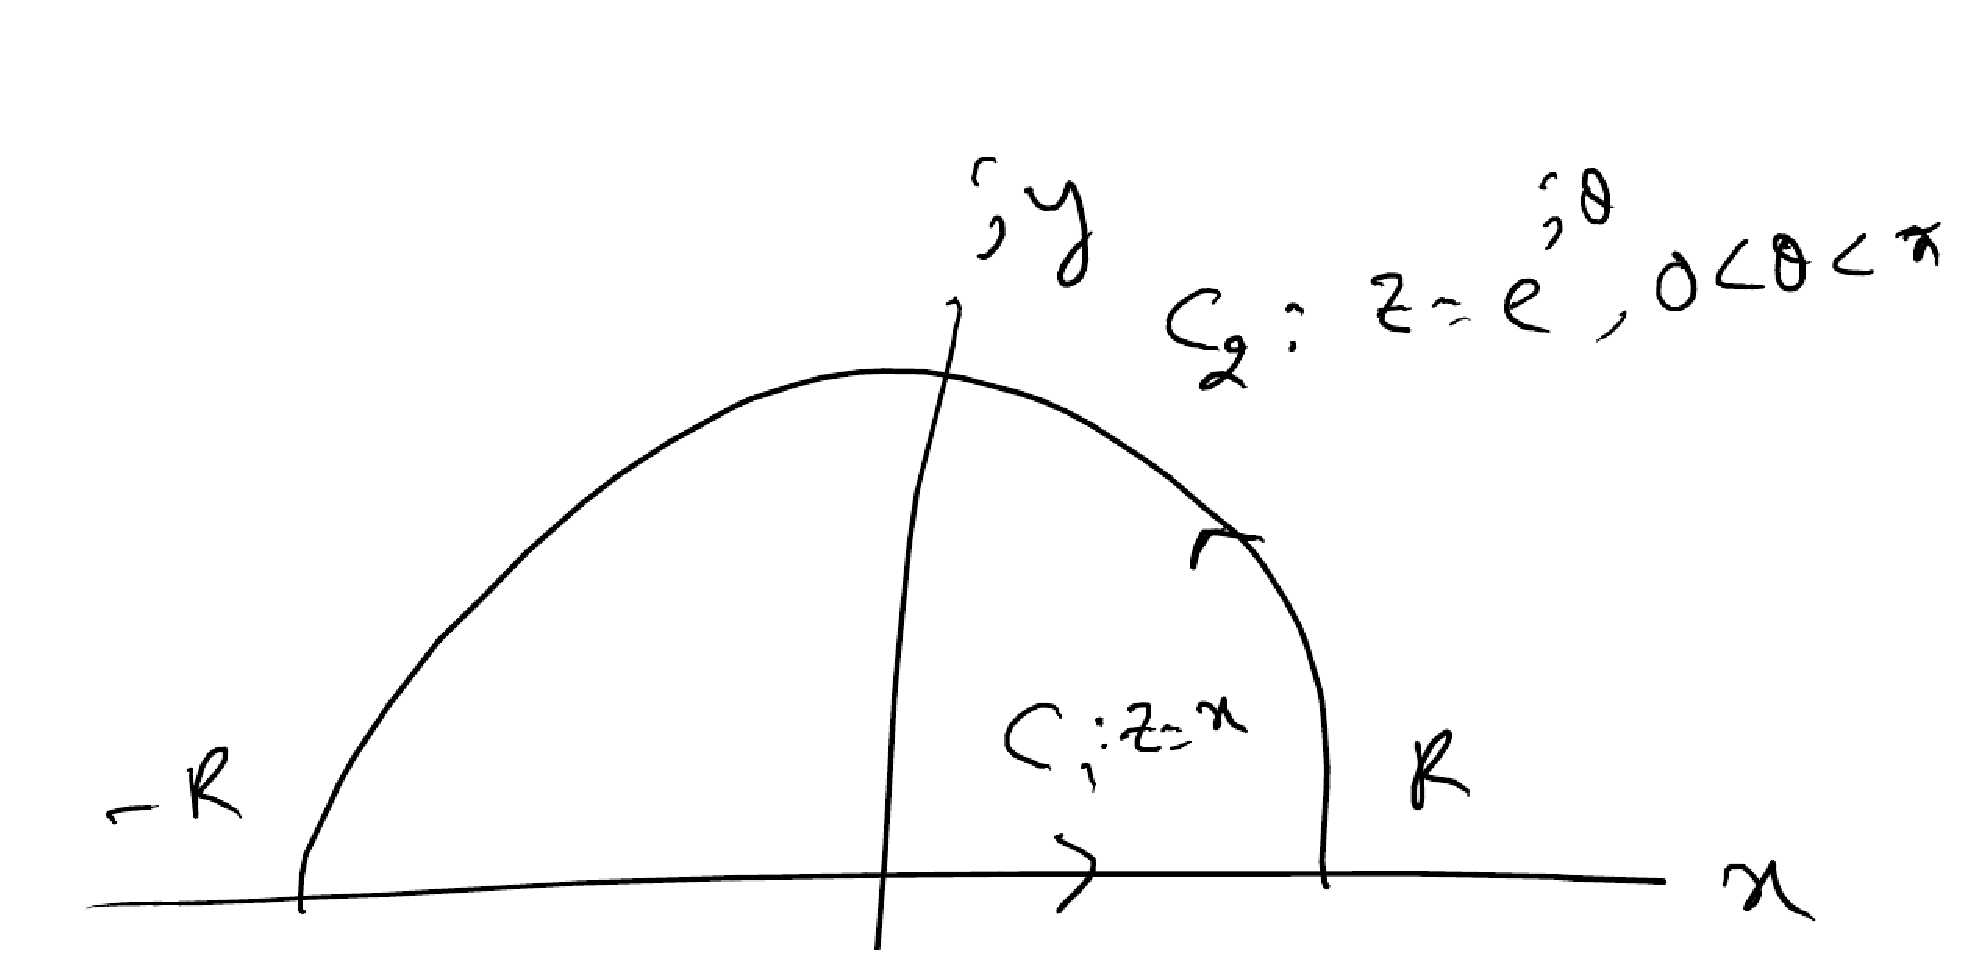
\includegraphics[width=\columnwidth]{./figs/contour.eps}
%\caption{}
%\label{fig:contour}
%\end{figure}
%%
%
%%\begin{figure}[!h]
%%\centering
%%\resizebox {\columnwidth} {!} {
%%%\documentclass[border=10mm]{standalone}
%\begin{document}
\begin{tikzpicture}
  
  \def\Radius{1.5}
  \path
    (-\Radius, 0) coordinate (A)
    -- coordinate (M)
    (\Radius, 0) coordinate (B)
    (M) +(60:\Radius) coordinate (C)
    +(120:\Radius) coordinate (D)
  ;
\draw[
        decoration={markings, mark=at position -0.84 with {\arrow{>}}},
        postaction={decorate}
        ]  
  (B) arc(0:180:\Radius) -- cycle
  ;
  
\draw[
        decoration={markings, mark=at position 0.9 with {\arrow{>}}},
        postaction={decorate}
        ]  
  (B) arc(0:180:\Radius) -- cycle
  ;
  
  
%these are axs:
\draw[arrows=<->](-2.5,0)--(2.5,0);
\draw[arrows=<->](0,-1.5) -- (0,2);
%these are points: 
  \put(45,4){\tiny $R$}
  \put(72,-1){\small $x$}
  \draw(0.9,-0.3) node{\tiny $C_1:\zst=x$};
  \put(-55,4){\tiny $-R$}
    \put(0,0){\tiny $O$}
    \put(0,45){\tiny ${\jmath}y$}
  
  %text rotation
\begin{turn}{35}
\draw (3,0.2) node {\tiny $C_2:\zst=e^{\jmath{\theta}},0<{\theta}<{\pi}$};
\end{turn}
    
\end{tikzpicture}
%\end{document}
%%}
%%\caption{}
%%\label{fig:contour}
%%\end{figure}
%\begin{problem}
%Show that
%\begin{equation}
%\lim_{R\to \infty}\abs{ \frac{e^{-\j zt}}{1+z^2}} = 0, \quad t < 0
%\end{equation}
%by substituting $z = Re^{\j \theta}, 0 < \theta < \pi$.
%\end{problem}
%%
%\begin{problem}
%Let $C$ be a closed curve within the curve $T$.  Then given that
%\begin{equation}
%\ointctrclockwise_C \frac{e^{-\j zt}}{1+z^2}\,dz = \ointctrclockwise_T \frac{e^{-\j zt}}{1+z^2}\,dz,
%\end{equation}
%show that
%\begin{equation}
%\ointctrclockwise_C \frac{e^{-\j zt}}{1+z^2}\,dz = \int_{-\infty}^{\infty} \frac{e^{-\j x t}}{1+x^2}\,dx, \quad t < 0
%\end{equation}
%\end{problem}
%\begin{problem}
%Given that
%\begin{equation}
%\ointctrclockwise_C \frac{f(z)}{z-z_0}\,dz = 2\pi \j f(z_0), 
%\end{equation}
%%
%where $z_0$ is within $C$, show that
%\begin{equation}
%\ointctrclockwise_C \frac{e^{-\j zt}}{1+z^2}\,dz = \pi e^t \quad t < 0
%\end{equation}
%\end{problem}
%\begin{problem}
%Now find 
%\begin{equation}
%\int_{-\infty}^{\infty} \frac{e^{-\j x t}}{1+x^2}\,dx, \quad t > 0
%\end{equation}
%\end{problem}
%%
%\begin{problem}
%Obtain an expression for the probability density function (PDF) of $X$.
%\end{problem}
%\section{Cauchy's Integral Formula}
%\begin{problem}
%Show that
%\begin{equation}
%\ointctrclockwise_C \frac{f(z)}{z-z_0}\,dz =  f(z_0)\ointctrclockwise_C \frac{dz}{z-z_0} + \ointctrclockwise_C \frac{f(z)-f(z_0)}{z-z_0}\,dz
%\end{equation}
%\end{problem}
%\begin{problem}
%For $C:z = z_0+\rho e^{\j\theta}, 0 < \theta < \pi$, show that
%\begin{equation}
%\ointctrclockwise_C \frac{dz}{z-z_0} = 2\pi \j
%\end{equation}
%\end{problem}
%%
%\begin{problem}
%Let
%\begin{equation}
%\abs{\frac{f(z)-f(z_0)}{z-z_0} - K} < \delta \implies \abs{z-z_0} < \epsilon
%\end{equation}
%for some $\epsilon, \delta > 0$.  
%\begin{enumerate}
%\item
%Show that 
%\begin{equation}
%\abs{f(z)-Kz -f(z_0)+Kz_0} < \epsilon\delta
%\end{equation}
%\item Let
%\begin{align}
%f_1(z) &=  f(z)-Kz
%\\
%f_2(z) &= Kz 
%\end{align}
%Show that 
%\begin{multline}
%\abs{f_1(z)+f_2(z)-f_1(z_0)-f_2(z_0)} 
%\\
%= \abs{f(z)-f(z_0)} < \kappa 
%\end{multline}
%%Let $f_1(z),f_2(z)$ be two functions such that
%%\begin{align}
%%\abs{f_1(z)-f_1(z_0)} < \delta_1 \implies \abs{z-z_0} < \epsilon_1
%%\\
%%\abs{f_1(z)-f_1(z_0)} < \delta_1 \implies \abs{z-z_0} < \epsilon_1
%%\end{align}
%\item Let
%\begin{equation}
%g(z)=\abs{\frac{f(z)-f(z_0)}{z-z_0} - K}
%\end{equation}
%\end{enumerate}
%%\begin{equation}
%%\abs{f(z)-f(z_0)} < \delta_1 \implies \abs{z-z_0} < \epsilon_1, \quad \epsilon_1, \delta_1 > 0
%%\end{equation}
%\end{problem}
%\begin{problem}
%Let 
%\begin{equation}
%\abs{g(z)} < \frac{\epsilon}{\rho}
%\end{equation}
%Show that, if $C:z = \rho e^{\j\theta}, 0 < \theta < 2\pi$ and $z_i \in C, \Delta z_m = z_m - z_{m-1}, \zeta_m \in \brak{z_{n-1},z_{n}}$,
%\begin{equation}
%\abs{\sum_{m=1}^{n}g(\zeta_m)\Delta z_m} < 2\pi\epsilon
%\end{equation}
%\end{problem}
%\begin{definition}
%\begin{equation}
%\label{eq:line_int_def}
%\int_C g(z)\,dz = \lim_{\substack{\Delta z_m \to 0 \\ n \to \infty}}\abs{\sum_{m=1}^{n}g(\zeta_m)\Delta z_m} 
%\end{equation}
%\end{definition}
%\begin{problem}
%Show that 
%\begin{equation}
%\abs{\int_C \frac{f(z)-f(z_0)}{z-z_0}\,dz} < 2\pi\epsilon
%\end{equation}
%%
%\end{problem}
%\begin{problem}
%Show that
%\begin{equation}
%\ointctrclockwise_C \frac{f(z)}{z-z_0}\,dz =  2\pi \j f(z_0)
%\end{equation}
%\end{problem}
%\section{Cauchy's Integral Theorem}
%\begin{definition}
% The  derivative of $f(z)$ is defined as
%\begin{equation}
%\lim_{\Delta z \to 0} \frac{f(z+\Delta z)-f(z)}{\Delta z}
%\end{equation}
%$f(z)$ is said to be {\em analytic} if its derivative exists.
%\end{definition}
%\begin{problem}
%Let $z = x + \j y, \Delta z = \Delta x + \Delta y, f(z) = u(x,y)+\j v(x,y)$. 
%\begin{enumerate}
%\item By letting $\Delta y \to 0$ followed by $\Delta x \to 0$, show that
%\begin{align}
%f^{\prime}(z) = \frac{\partial u}{\partial x} + \j \frac{\partial v}{\partial x}
%\end{align}
%\item By letting $\Delta x \to 0$ followed by $\Delta y \to 0$, show that
%\begin{align}
%f^{\prime}(z) = \frac{\partial v}{\partial y} - \j \frac{\partial u}{\partial y}
%\end{align}
%\end{enumerate}
%\end{problem}
%\begin{problem}
%Show that
%\begin{align}
%\frac{\partial u}{\partial x} &= \frac{\partial v}{\partial y}
%\\
%\frac{\partial u}{\partial y} &= -\frac{\partial v}{\partial x}
%\end{align}
%These are known as the {\em Cauchy-Riemann} equations.
%\end{problem}
%%
%\begin{problem}
%Using \eqref{eq:line_int_def}, show that
%\begin{multline}
%\oint_{C}f(z)\,dz = \oint_{C}\brak{u\,dx- v\,dy }
%\\
%+ \j \oint_{C}\brak{u\,dy+v\,dx}
%\end{multline}
%\end{problem}
%\begin{problem}
%According to {\em Green's Theorem}, for a closed curve $C$,
%\begin{equation}
%\oint_{C}\brak{u\,dx- v\,dy} = \iint_{R} \brak{-\frac{\partial v}{\partial x}-\frac{\partial u}{\partial y}}\,dx\,dy
%\end{equation}
%where $R$ is bounded by $C$.  Show that
%\begin{equation}
%\oint_{C}f(z)\,dz  = 0.
%\end{equation}
%assuming that $f(z)$ is analytic everywhere inside $C$.
%\end{problem}
%%
%\begin{problem}
%In Fig. \ref{fig:CT},  show that 
%\begin{equation}
%\oint_{C}f(z)\,dz = \oint_{T}f(z)\,dz
%\end{equation}
%given that $f(z)$ is analytic in the region between $C-T$.
%\end{problem}
%\begin{figure}[!h]
%\centering
%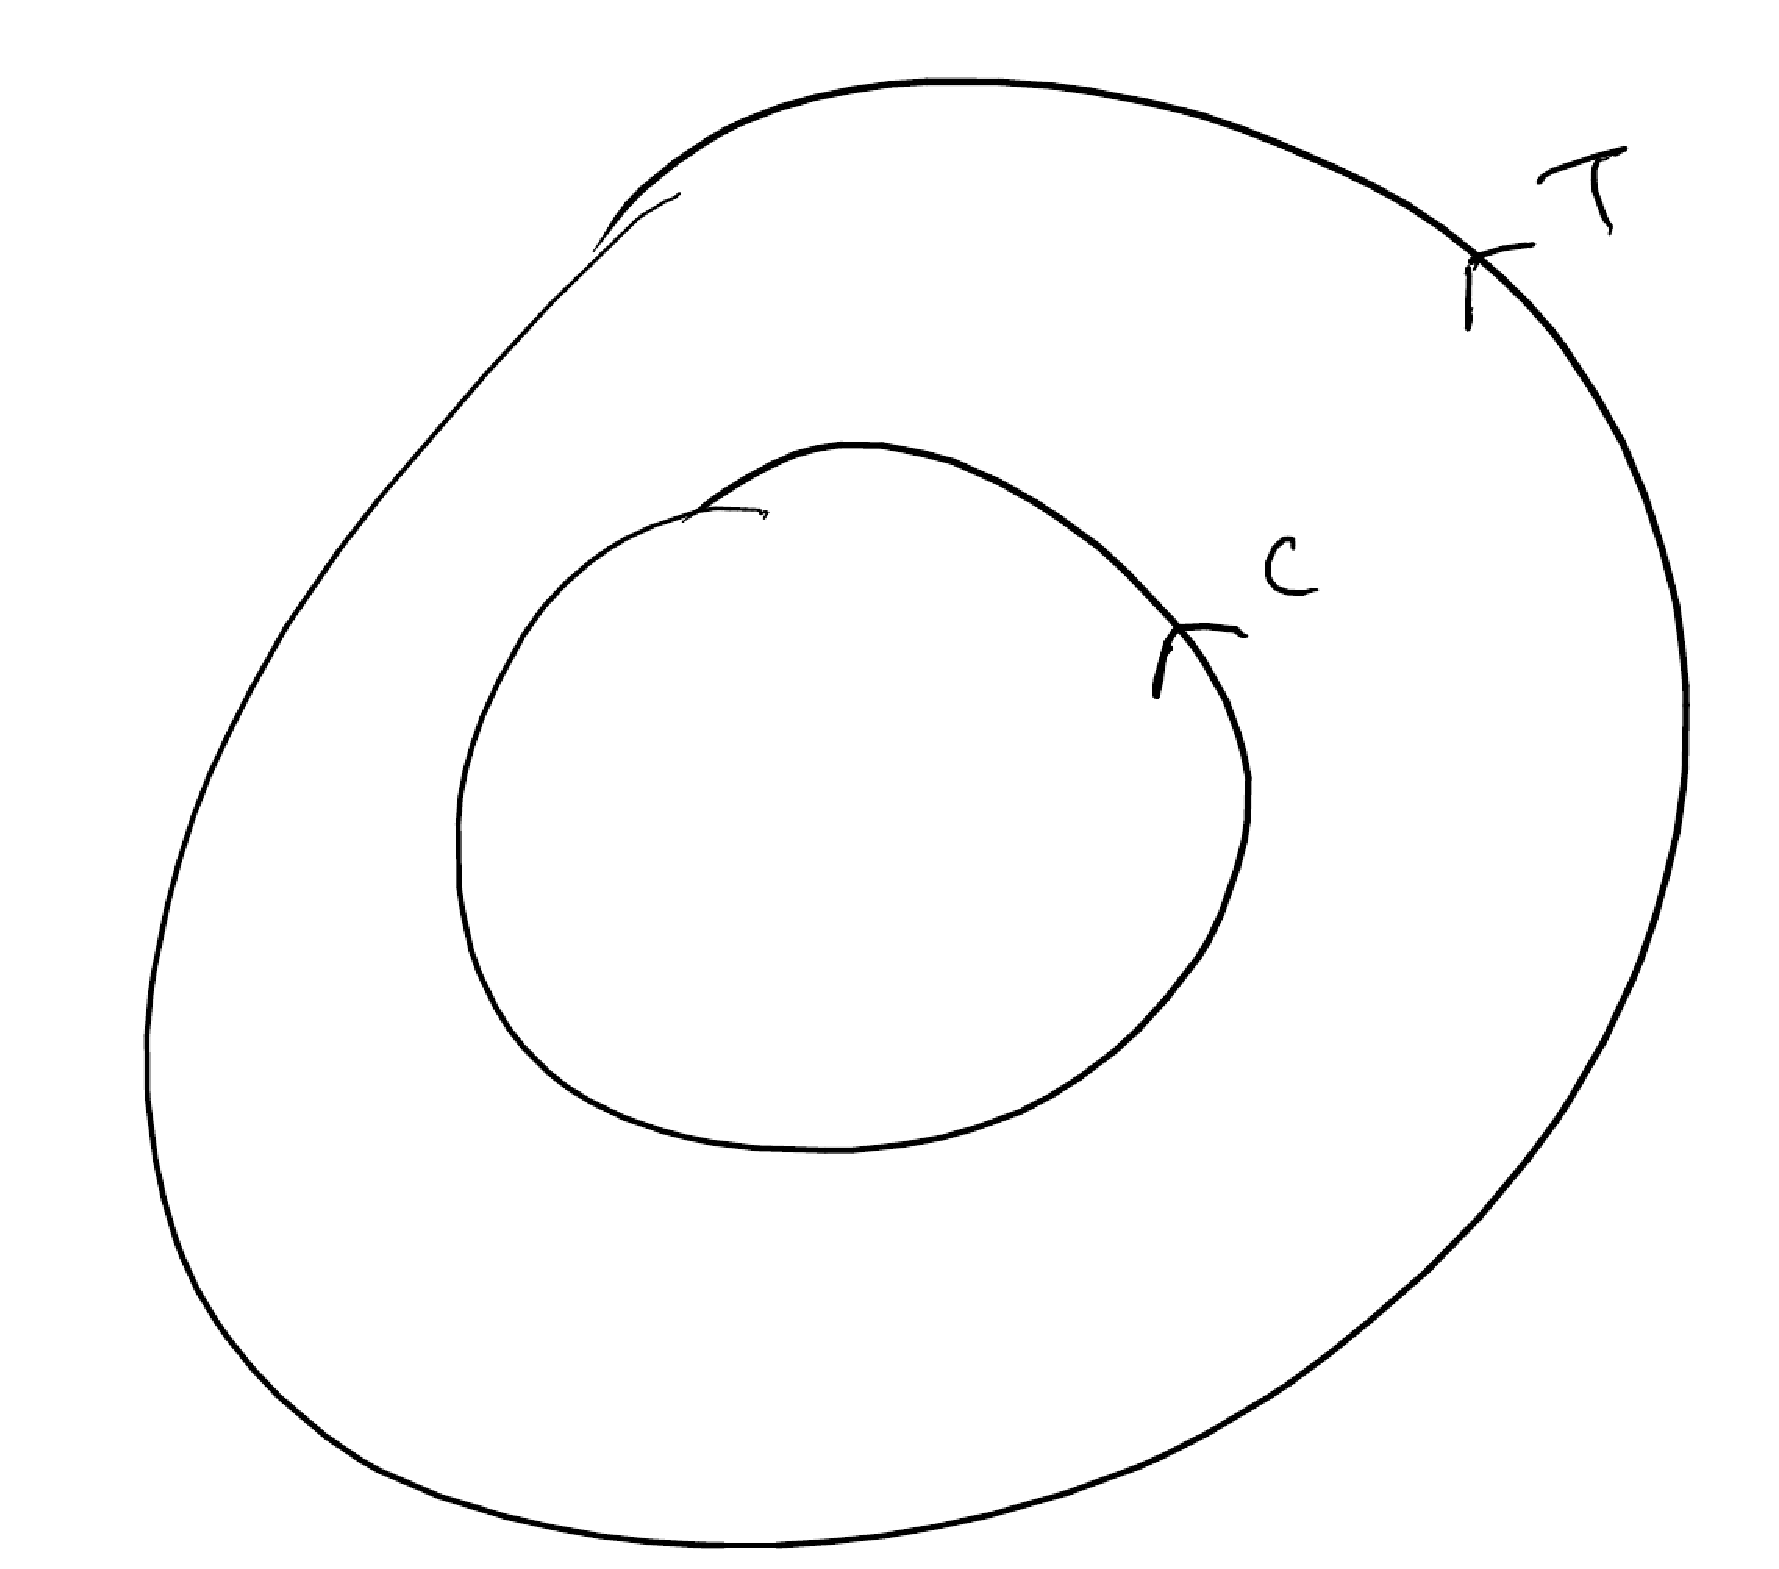
\includegraphics[width=\columnwidth]{./figs/CT.eps}
%\caption{}
%\label{fig:CT}
%\end{figure}
%
%\begin{problem}
%The PDf of an exponential random variable $X$ is defined as
%%
%\begin{equation}
%p_{X}(t) = 
%\begin{cases}
%\frac{1}{\gamma}e^{-\frac{t}{\gamma}} & t \geq 0 \\
%0 & t < 0
%\end{cases}
%\end{equation}
%%
%\begin{enumerate}
%\item The {\em expectation} of the function $g(X)$ is defined as
%%
%\begin{equation}
%E\sbrak{g(X)} = \int_{\infty}^{\infty} g(t)p_V(t)\, dt
%\end{equation}
%%
%Find $E\sbrak{X}$.
%\item The cumulative distribution function (CDF) of $X$ is defined as $F_X(t)=\pr{X > t}$.  Show that the CDF of $X$ is
%\begin{equation}
%\label{cdf_exp}
%F_X(t) = 
%\begin{cases}
%1 - e^{-\frac{t}{\gamma}} & t \geq 0 \\
%0 & t < 0
%\end{cases}
%\end{equation}
%\item The characteristic function of $X$ is defined as $\phi_X(\j \omega)=E\sbrak{e^{\j \omega X}}$.  Show that
%%
%\begin{equation}
%\label{cf_exp}
%\phi_{X}\brak{\j \omega} = \frac{1}{1 - \j \omega \gamma}
%\end{equation}
%%
%\item The moment generating function (MGF) of $X$ is defined as $E\sbrak{e^{-s  X}}$.  Show that
%%
%\begin{equation}
%M_{X}\brak{s} = \frac{1}{1 + s \gamma}
%\end{equation}
%%
%\end{enumerate}
%\end{problem}
%%
%\begin{problem}
%The PDF of $X$ can be {\em recovered} from the CF using the following formula
%%
%\begin{equation}
%p_{X}(x) = \frac{1}{2\pi}\int_{-\infty}^{\infty}\phi_{X}\brak{\j\omega}e^{-\j \omega x}d\omega
%\label{pdf_inv_exp}
%\end{equation}
%since the PDF and CF are governed by the {\em Fourier Transform} relationship.
%%
%\begin{enumerate}
%\item Show that  $p_{X}$  in \eqref{pdf_inv_exp} can be expressed as
%\begin{equation}
%p_{X}(t) = \frac{1}{2\pi \j}\int_{-\j\infty}^{\j\infty}\frac{f(z)}{1 - z \gamma}dz
%%\label{pdf_inv_exp}
%\end{equation}
%where $f(z) = e^{-zt}$.
%\item Let $z = x + \j y$, where $x$ and $y$ are real variables. If $f(z) =  u(x,y)+\j v(x,y)$, show that
%%
%\begin{equation}
%\begin{split}
%u(x,y) &= e^{-xt}\cos(ty) \\
%v(x,y) &= -e^{-xt}\sin(ty) \\
%\end{split}
%\end{equation}
%%
%\item Show that
%\begin{equation}
%\begin{split}{\frac {\partial u}{\partial x}}&={\frac {\partial v}{\partial y}}
%\\
%{\frac {\partial u}{\partial y}}&=-{\frac {\partial v}{\partial x}}\end{split}
%\end{equation}
%The above equations are known as the {\em Cauchy-Reimann} equations and any function $f$ that satisfies the above equations is known as an {\em Analytic function}.
%\item Let $C$ be the unit circle with centre at $\frac{1}{\gamma}$ defined as $C:z = \frac{1}{\gamma} + e^{\j \theta}, 0 < \theta < 2\pi$. Show that
%%
%\begin{equation}
%\ointctrclockwise_{C}\frac{dz}{1-z\gamma} = -\frac{2\pi\j}{\gamma}
%\end{equation}
%%
%through a change of variables in terms of $\theta$.  The integral on the L.H.S. above is known as a {\em contour integral}.  Note that the direction of integration is clockwise.
%\item Let 
%\begin{equation}
%g(z) = \frac{f(z) - f\brak{\frac{1}{\gamma}}}{z - \frac{1}{\gamma}}
%\end{equation}
%%
%Show that $g(z)$ is analytic for $z \neq \frac{1}{\gamma}$.
%\item An analytic function is also continuous. Show that
%%\begin{enumerate}
% $\abs{g(z)} < \frac{\epsilon}{\delta}$
%\item Let $K: z = \frac{1}{\gamma} + \rho e^{\j \theta}, 0 < \theta \leq 2\pi $.  If 
%%
%\begin{equation}
%\ointctrclockwise_{K}g(z)\,dz \triangleq \sum_{k} g(z_k)\Delta z_k,
%\end{equation}
%%
%show that 
%%
%\begin{equation}
%\abs{\ointctrclockwise_{K} g(z)} < 2\pi \epsilon
%\end{equation}
%%
%\item If 
%\begin{equation}
%\ointctrclockwise_{C}\frac{f(z)}{1 - z \gamma}dz = \ointctrclockwise_{K}\frac{f(z)}{1 - z \gamma}dz,
%\end{equation}
%show that
%\begin{equation}
%\ointctrclockwise_{C}\frac{f(z)}{1 - z \gamma}dz = -\frac{2\pi\j}{\gamma}f\brak{\frac{1}{\gamma}}
%\end{equation}
%\item Let $D: R e^{\j \theta}, -\frac{\pi}{2} < \theta < \frac{\pi}{2}$.  Show that
%%
%\begin{equation}
%\lim_{R \rightarrow \infty} \int_{D}\frac{f(z)}{1 - z \gamma}dz = 0
%\end{equation}
%%
%\item Show that
%%
%\begin{align}
%p_{X}(t) = \frac{1}{\gamma} e^{-\frac{t}{\gamma}} \quad  t \geq 0
%\end{align}
%%
%\item Show that
%%
%\begin{align}
%p_{X}(t) = 0  \quad  t < 0
%\end{align}
%%
%\end{enumerate}
%%
%%
%%\end{enumerate} 
%\end{problem}
%%
%\begin{problem}
%\begin{enumerate}
%The Fourier transform of the unit step function $u(t)$ is
%%
%\begin{align}
%\int_{-\infty}^{\infty}u(t)e^{\j\omega t} = \frac{\delta(\omega)}{2} +\frac{\j}{\omega}
%\end{align}
%%
%\item Show that the CDF of a random variable $X$ can be expressed in terms of its CF
%$\phi_{X}\brak{\omega}$ as
%%
%\begin{align}
%\label{gil}
%F_{X}(x) = \frac{1}{2}-\frac{1}{2\pi\j}\int_{-\infty}^{\infty}\frac{\phi_{X}\brak{\omega}}{\omega}e^{-\j\omega x}\,d\omega
%\end{align}
%This is known as the Gil-Pelaez formula.
%%\item Show that
%%\begin{equation}
%%F_{X}(x)={\frac {1}{2}}-{\frac {1}{\pi }}\int _{0}^{\infty }{\frac {\operatorname {Im} [e^{-\j tx}\phi _{X}(t)]}{t}}\,dt.
%%\end{equation}
%\item Using the above relation, obtain the CDF in  \eqref{cdf_exp} using contour integration.  You may express \eqref{gil} as
%\begin{multline}
%\label{gilpv}
%F_{X}(x) = \frac{1}{2}-\frac{1}{2\pi\j}\lim_{\substack {r\rightarrow 0 \\ R\rightarrow \infty} }\lsbrak{\int_{-R}^{r}\frac{\phi_{X}\brak{\omega}}{\omega}e^{-\j\omega x}\,d\omega} 
%\\
%+ \rsbrak{\int_{r}^{R}\frac{\phi_{X}\brak{\omega}}{\omega}e^{-\j\omega x}\,d\omega}
%\end{multline}
%\end{enumerate}
%\end{problem}
%\begin{problem}
%Repeat the above exercises using the MGF instead of the CDF
%\end{problem}
%The Moment Generating Function (MGF) of $X$ is defined as
%%
%\begin{align}
%M_{X}(s) = E\sbrak{e^{s X}}
%\end{align}
%%
%where $X$ is a random variable and $E\sbrak{\cdot}$ is the expectation.  
%%
%%
%\begin{enumerate}
%\item Let $Y \sim \gauss{0}{1}$.  Define
%%
%\begin{align}
%Q(x) = \pr{Y > x}, x > 0
%\end{align}
%%
%Show that
%\begin{equation}
%Q(x) = \frac{1}{\pi}\int^{\frac{\pi}{2}}_{0}e^{-\frac{x^2}{2\sin^2 \theta}}\,d\theta
%\end{equation}
%\item 
%Let $h\sim\mathcal{CN}\brak{0,\frac{\Omega}{2}},n\sim\mathcal{CN}\brak{0,\frac{N_0}{2}}$.  Find the distribution of $\abs{h}^2$.

%\item Let
%%
%\begin{align}
%P_e = \pr{\Re \cbrak{h^*y} < 0}, \text{ where } y = \brak{\sqrt{E_s}h + n},
%\end{align}
%%
%Show that
%%
%\begin{align}
%P_e = \int_{0}^{\infty}\qfunc{\sqrt{2x}}p_{A}(x) \,dx
%\end{align}
%where $A = \frac{E_s\abs{h}^2}{N_0}$.
%\item Show that
%%
%\begin{align}
%P_e 
%%&= E\sbrak{\qfunc{\sqrt{2A}}} \\
%%&=  \frac{1}{\pi}\int_{0}^{\frac{\pi}{2}}E\sbrak{e^{-\frac{A}{\sin^2\theta}}}\,d\theta \\
%&=  \frac{1}{\pi}\int_{0}^{\frac{\pi}{2}}M_{A}\brak{-\frac{1}{\sin^2\theta}}\,d\theta
%\label{ch4_pe_mgf}
%\end{align}
%%
%\item compute $M_A(s)$.
%%
%\item 
%Find $P_e$.
%\item 
%If $\gamma = \frac{\Omega E_s}{N_0}$, show that $P_e < \frac{1}{2\gamma}$. 
%\end{enumerate}
%\end{problem}
%%
%\begin{problem}
%Find
%%
%\begin{align}
%\frac{1}{\gamma}\int_{0}^{\infty}\qfunc{\sqrt{2x}}e^{-\frac{x}{\gamma}} \,dx
%\end{align}
%%
%\end{problem}
%\begin{problem}
%Tthe characteristic function (CF) of a random variable $X$ is defined as
%%
%\begin{align}
%\phi_{X}(\omega) = E\sbrak{e^{\j \omega X}}
%\end{align}
%%
%where $X$ is a random variable and $E\sbrak{\cdot}$ is the expectation.  Show that the characteristic function of $V$, given that its PDF
%%
%\begin{align}
%p_{V}(x)= \frac{1}{\gamma}e^{-\frac{x}{\gamma}}, \quad x > 0, \gamma > 0
%\end{align}
%%
%is
%%
%\begin{align}
%\phi_{V}\brak{\omega} 
%%&= \frac{1}{\gamma}\int_{0}^{\infty}e^{\j\omega v}e^{-v/\gamma}\,dv \\
%%&= \frac{1}{\gamma}\int_{0}^{\infty}e^{-v\brak{1/\gamma -\j\omega}}\,dv \\
%&= \frac{1}{1-\j\omega\gamma}
%\end{align}
%%
%\end{problem}
%\begin{problem}
%Show that the charactersitic function of $X^2$, where $X \sim \mathcal{N}\brak{0,1}$
%is
%%
%\begin{align}
%\phi_{X^2}\brak{\omega} = \frac{1}{\brak{1-2\j\omega}^{\frac{1}{2}}}
%\end{align}
%%
%\end{problem}
%\begin{problem}
%Find the characteristic function of 
%%
%\begin{align}
%D = X^2-V
%\end{align}
%\end{problem}
%\begin{problem}
%Find $A$ and $B$ such that
%%
%\begin{align}
%A &= \sbrak{\phi_{X}\brak{\omega}}_{\omega = 0} \\
%B &= \sbrak{\brak{\omega - \frac{j}{\gamma}}\frac{\phi_{X}\brak{\omega}}{\omega}}_{\omega = \frac{\j}{\gamma}}
%\end{align}
%%
%Evaluate
%%
%\begin{align}
%\frac{1}{2}\sbrak{\frac{1}{2} + \frac{1}{2\pi\j}\brak{\j\pi A + 2\pi \j B}}
%\end{align}
%%
%Comment.
%\end{problem}
%\begin{problem}
%The Fourier transform of the unit step function $u(t)$ is
%%
%\begin{align}
%\int_{-\infty}^{\infty}u(t)e^{\j\omega t} = \frac{\delta(\omega)}{2} +\frac{\j}{\omega}
%\end{align}
%%
%Show that the CDF of a random variable $X$ can be expressed in terms of its CF
%$\phi_{X}\brak{\omega}$ as
%%
%\begin{align}
%F_{X}(x) = \frac{1}{2}-\frac{1}{2\pi\j}\int_{-\infty}^{\infty}\frac{\phi_{X}\brak{\omega}}{\omega}e^{-\j\omega x}\,d\omega
%\end{align}
%%
%\end{problem}
%%
%\begin{problem}
%Show that
%%
%\begin{equation}
%Q(x) = \frac{1}{\pi}\int_{0}^{\frac{\pi}{2}}e^{-\frac{y^2}{2\sin^2 \theta}}\,d\theta
%\end{equation}
%%
%This is an alternative expression for the $Q$-function.
%\end{problem}

%\input{./chapter1/ch1}
%
%\newpage
%\section{Application}
%\input{./chapter2/ch2}
%\newpage
%\section{Binary Modulation}
%\input{chapter2} 
%
%\newpage
%\section{$M$-ary Modulation}
%\input{chapter3} 

%\newpage
%\section{BER in Rayleigh Flat Slowly Fading Channels}
%\input{chapter4} 

\end{document}


